% =============================================================================
% The CGAL Developers' Manual
% Chapter: Specification Documentation
% -----------------------------------------------------------------------------
% file   : specification.tex
% authors: Susan Hert <hert@mpi-sb.mpg.de>
% -----------------------------------------------------------------------------
% $Revision$
% $Date$
% =============================================================================

\chapter{Specification Documentation}
\label{chap:specification}

\ccIndexMainItemBegin{manuals}
\ccChapterRelease{Chapter Version: 1.1} \\
\ccChapterAuthor{Susan Hert ({\tt hert@mpi-sb.mpg.de})}

The official \cgal\ 
\ccAnchor{http://www.cgal.org/Manual/}{documentation} 
is currently divided into six separate manuals:
\begin{itemize}
   \item \ccAnchor{http://www.cgal.org/Manual/doc_html/installation/contents.html}{Installation Guide}
   \item \ccAnchor{http://www.cgal.org/Manual/doc_html/ref-manual0/contents.html}{General Introduction}
   \item \ccAnchor{http://www.cgal.org/Manual/doc_html/ref-manual1/contents.html}{Kernel}
   \item \ccAnchor{http://www.cgal.org/Manual/doc_html/ref-manual2/contents.html}{Basic Library}
   \item \ccAnchor{http://www.cgal.org/Manual/doc_html/ref-manual3/contents.html}{Support Library}
   \item \ccAnchor{http://www.cgal.org/Manual/doc_html/use_of_stl/contents.html}{Use of \stl\ and \stl\ Extensions in \cgal}
\end{itemize}
Not surprisingly, the Installation Guide describes how to install \cgal
\ccIndexMainItem{installation}, 
and the General Introduction generally introduces the library 
by discussing the organization of the manuals
\ccIndexSubitem{manuals}{organization}, the
\cgal\ namespace (Chapter~\ref{chap:namespaces}),
\ccIndexSubitem{namespace}{\ccFont CGAL} restrictions on the 
inclusion order of header files
\ccIndexSubitem{header files}{inclusion order},
changes since the last release
\ccIndexMainItem{release changes}
and the various checks (preconditions,
postconditions, {\em etc.}; see Chapter~\ref{chap:checks})
\ccIndexMainItem{preconditions}
\ccIndexMainItem{postconditions}
\ccIndexMainItem{assertions}
\ccIndexMainItem{warnings}
used in the library.
(This manual began its life as a larger document, but the information 
originally contained in it has since been farmed out to other manuals.
When someone has the time to attend to it, this manual should grow again
to include a broader overview of the library.) The Use of \stl\ manual
describes features of \stl\
\ccIndexMainItem{\stl} that are used and extended in \cgal.

Documentation of new packages and features will likely be included in
the Kernel, Basic Library, and Support Library documentation.  See 
Section~\ref{sec:overall_design} for a description of what these three 
parts of the library contain. Each of
these manuals is (or, rather, will soon be) further subdivided into two 
parts:  a Reference Manual and a Users' Manual.  Sections~\ref{sec:ref_manual}
and~\ref{sec:users_manual} below describe the contents of these two parts.

The manuals are produced from \ccTexHtml{\LaTeX\ }{LaTeX} input files in 
both PostScript and
HTML format.  The conversion from \ccTexHtml{\LaTeX\ }{LaTeX} input to HTML 
output is accomplished 
through the use of a set of shell scripts and programs, as well as style 
files that were designed to support this conversion.  These style files
provide numerous commands that are used to format the manuals in a
(more or less) uniform fashion.  Section~\ref{sec:manual_tools}
provides the basic information about these tools and style files that 
you will need to produce documentation of your package specification.
Section~\ref{sec:files_required} describes the files that 
are required for submitting documentation.  Sections~\ref{sec:doc_figures}
and~\ref{sec:indexing} give information about including figures in your
documentation and inserting indexing commands, respectively.  The conversion
to HTML is briefly discussed in Section~\ref{sec:html_conversion}.  
Section~\ref{sec:doc_test_suite} describes the manual test suite run
for each internal release of the library.  Common problems and solutions
are described in Section~\ref{sec:common_problems} followed by a section
summarizing the requirements and recommendations for specification 
documentation.

\section{The manual tools}
\label{sec:manual_tools}
\ccModifierCrossRefOff
\ccIndexSubitemBegin{tools}{manual}

The manual tools are provided as a compressed tar file that is downloadable
from \path|http://www.mpi-sb.mpg.de/~hert/CGAL/Tools/|.  When unpacked, the
tar file will create a directory called {\tt Tools} that contains the following
subdirectories:

\begin{description}
   \item[{\bf\tt doc/}] -- directory containing the documentation for
        the tools
   \item[{\bf\tt example/}] -- directory containing example documentation
   \item[{\bf\tt format/}] -- directory containing the 
        \ccTexHtml{\LaTeX\ }{LaTeX} style files
        used for formatting the manual
   \item[{\bf\tt scripts/}] -- directory containing the various scripts
        to do conversions
   \item[{\bf\tt src/}] -- directory containing the style files and program
        source code for the tools used to convert from 
        \ccTexHtml{\LaTeX\ }{LaTeX} to HTML.
\end{description}

There are also {\tt README} and {\tt INSTALLATION} files provided that
will help you to install the tools on your system.

\subsection{The style files}
\label{subsec:manual_style_files}
\ccIndexSubsubitem{tools}{manual}{style files}

The manuals are developed through the use of the style files 
{\tt cc\_manual.sty}\ccIndexMainItem[c]{\tt cc_manual.sty} and 
{\tt cc\_manual\_index.sty}\ccIndexMainItem[c]{\tt cc_manual_index.sty}
that provide formatting
commands and style file {\tt latex\_converter.sty}
\ccIndexMainItem[c]{\tt latex_converter.sty}
that provides commands
useful for the conversion to HTML.  
For each of these files, there is a PostScript document describing 
the file, the commands it defines, and how to use them.  These documents 
(\ccAnchor{./cc_manual.ps.gz}{{\tt cc\_manual.ps.gz}}, 
\ccAnchor{./cc_manual_index.ps.gz}{{\tt cc\_manual\_index.ps.gz}} and
\ccAnchor{./latex_to_html.ps.gz}{{\tt latex\_to\_html.ps.gz}}, respectively)
are located in the {\tt Tools/doc} 
directory\ccIndexSubsubitem{tools}{manual}{documentation}.

\subsection{Scripts and programs}
\label{sec:manual_scripts}
\ccIndexSubsubitem{tools}{manual}{scripts}
\ccIndexSubsubitem{tools}{manual}{programs}

The following scripts and programs are provided with the tools package.

\begin{itemize}
         \lcRawHtml{<A NAME="add_part_num">}
   \item \verb|add_part_num|\lcRawHtml{</A>}%
         \index{add_part_num script@{\tt add\_part\_num} script}%
         \ccIndexSubitem{index}{adding part number to}
         -- script used to prepend a part number to the 
         page numbers in a {\tt .idx} file produced by the indexing commands in
         a \ccTexHtml{\LaTeX\ }{LaTeX} document.  
         See \ccAnchor{./cc_manual_index.ps.gz}{{\tt Tools/doc/cc\_manual\_index.ps.gz}}.
   \item \lcRawHtml{<A NAME="cc_extract_html">} 
         \verb|cc_extract_html|\lcRawHtml{</A>}%
         \index{cc_extract_html program@{\tt cc\_extract\_html} program}%
          -- program used by {\tt cc\_manual\_to\_html}
         that converts a \ccTexHtml{\LaTeX\ }{LaTeX} file into an HTML file.
         See \ccAnchor{./latex_to_html.ps.gz}{{\tt Tools/doc/latex\_to\_html.ps.gz}}.
         \lcRawHtml{<A NAME="cc_extract_images">}
   \item \verb|cc_extract_images|\lcRawHtml{</A>}%
         \index{cc_extract_images program@{\tt cc\_extract\_images} program}
         -- program used by {\tt cc\_manual\_to\_html}
         that extracts inline images
         ({\tt .gif} files) from an HTML stream given on \ccc{stdin}.
         \lcRawHtml{<A NAME="cc_extract_include">}
   \item \verb|cc_extract_include|\lcRawHtml{</A>}%
         \index{cc_extract_include script@{\tt cc\_extract\_include} script}
         -- script to extract \verb|\ccInclude|
         statements from a specification file and write these converted to
         C preprocessor includes to standard output.  
         \lcRawHtml{<A NAME="cc_make_ref_pages">}
   \item \verb|cc_make_ref_pages|\lcRawHtml{</A>}
         \index{cc_make_ref_pages script@{\tt cc\_make\_ref\_pages} script}
         -- script that creates a%
         \ccAnchor{example/doc_tex/basic/Package/Package_ref/main_tex}%
                  {{\tt main.tex}}%
         \ccIndexMainItem{\tt main.tex}%
         \ccIndexSubitem{reference manual}{\tt main.tex}
         file in a directory, the name of which is supplied as an argument.  
         This {\tt main.tex} will be the driver file for the reference manual 
         chapter for the directory named in the argument. See 
         \ccAnchor{./latex_to_html.ps.gz}{{\tt Tools/doc/cc\_manual.ps.gz}} 
         and the script itself for further explanation.
         \lcRawHtml{<A NAME="cc_manual_to_html">}
   \item \verb|cc_manual_to_html|\lcRawHtml{</A>}%
         \index{cc_manual_to_html script@{\tt cc\_manual\_to\_html} script}%
         -- script that does the conversion from \ccTexHtml{\LaTeX\ }{LaTeX} 
            to HTML\ccIndexSubitem{manuals}{HTML}%
            \ccIndexSubitem{manuals}{HTML}.  
            See \ccAnchor{./latex_to_html.ps.gz}{{\tt Tools/doc/latex\_to\_html.ps.gz}}%
         and \ccAnchor{./cc_manual.ps.gz}{{\tt Tools/doc/cc\_manual.ps.gz}}.
         \lcRawHtml{<A NAME="cc_ref_wizard">}
   \item \verb|cc_ref_wizard|\lcRawHtml{</A>}%
         \index{cc_ref_wizard script@{\tt cc\_ref\_wizard} script}
         -- script that creates a reference page skeleton%
         \ccIndexSubitem{reference manual}{page template script}%
         given the category of the item and the item name. See
         \ccAnchor{./cc_manual.ps.gz}{{\tt Tools/doc/cc\_manual.ps.gz}}
         and the script itself for further explanation.
         \lcRawHtml{<A NAME="cc_index_fix">}
   \item \verb|index_fix|\lcRawHtml{</A>}%
         \index{index_fix script@{\tt index\_fix} script}%
         \ccIndexSubitem{index}{postprocessing}
         -- script used to postprocess an {\tt .ind } file 
         produced by {\tt makeindex} to make the index fit the specifications
         detailed in \ccAnchor{./cc_manual_index.ps.gz}%
         {{\tt Tools/doc/cc\_manual\_index.ps.gz}}.
\end{itemize}


The following programs are obsolete and will likely disappear from the
tools package:
\begin{itemize}
         \lcRawHtml{<A NAME="cc_extract">}
   \item \verb|cc_extract|\lcRawHtml{</A>}%
         \index{cc_extract program@{\tt cc\_extract} program}
          -- program to read a specification written with
         the \verb|cc_manual.sty| file and output all declarations in the
         document to standard output in \CC\ format. 
         See \ccAnchor{./cc_extract.ps.gz}{{\tt Tools/doc/cc\_extract.ps.gz}} for further explanation.
         \lcRawHtml{<A NAME="cc_check">}
   \item \verb|cc_check|\lcRawHtml{</A>}%
         \index{cc_extract script@{\tt cc\_check} script}
         -- script to check the consistency between a 
         specification written in a \ccTexHtml{\TeX\ }{TeX} file with the 
         \verb|cc_manual.sty| 
         and the implementation in a C++ header file.  See
         \ccAnchor{./cc_extract.ps.gz}{{\tt Tools/doc/cc\_extract.ps.gz}} 
         for further explanation.
         \lcRawHtml{<A NAME="cc_rename_include">}
   \item \verb|cc_rename_include|\lcRawHtml{</A>}%
         \index{cc_rename_include@{\tt cc\_rename\_include} script}
         -- script that renames all 
         \verb|\ccc{#include<...>}| directives in a document to 
         \verb|\ccInclude{...}| commands.  
         \lcRawHtml{<A NAME="cc_update_2.1">}
   \item \verb|cc_update_2.1|\lcRawHtml{</A>}%
         \index{cc_update_2.1 script@{\tt cc\_update\_2.1} script}
         -- script that can be used to translate a 
         document written using a version of the tools older than 2.1
         to the newer version. 
\end{itemize}
\ccIndexSubitemEnd{tools}{manual}
\ccModifierCrossRefOn

\section{Files required}
\label{sec:files_required}
\ccIndexSubitemBegin{manuals}{source files}
\ccIndexSubitemBegin{source files}{documentation}

Generally, each package in the library will have its own chapter in
both the reference manual and the users' manual%
\ccIndexMainItem{reference manual}%
\ccIndexMainItem{reference manual}, so you should write
your documentation accordingly.  That is, you should begin the documentation
for each of these parts with a \verb|\chapter| command. (Note, however, that
until the new manual style is used, the reference manual pages will not be 
put in their own chapter.)\ccIndexSubitem{manuals}{new style}

\ccIndexSubitem{directory structure}{for documentation}
It is required that the documentation submitted with a package be organized
according to a specific directory structure, which is described more
completely in Section~\ref{sec:doc_tex_subdirectory}.  You must submit
both the {\tt .tex} source files and a PostScript version of the reference
manual and users' manual chapters for your package according to the following
rules:
\begin{itemize}  
   \item The {\tt .tex} files for the users' manual%
         \ccIndexSubitem{users' manual}{directory} should be placed in a 
         directory \verb|doc_tex|/\VarText{manual part}/\VarText{Package}%
         \index{doc_tex directory@{\tt doc\_tex} directory}
         and must include a file 
         \ccAnchor{example/doc_tex/basic/Package/main_tex}{{\tt main.tex}}%
         \ccIndexMainItem{\tt main.tex}%
         \ccIndexSubitem{users' manual}{\tt main.tex} 
         that inputs all other users' 
         manual source files using the \verb|\input| command (NOT the
         \verb|\include| command).%
         \index{input@$\backslash${\tt input}!vs. include@vs. $\backslash${\tt include}}.
         (Until the new manual style is used, this
         file should also input the reference manual source files.)%
         \ccIndexSubitem{manuals}{new style}%
         \ccIndexMainItem{reference manual}

   \item The source files for the reference manual should be placed in the 
         directory \verb|doc_tex/|\VarText{manual part}/\VarText{Package}/%
         \VarText{Package}\verb|_ref|%
         \ccIndexSubitem{directory structure}{for reference manual}%
         \ccIndexSubitem{reference manual}{directory}%
         \index{ref directory@{\tt \_ref} directory}%
         (See Section~\ref{sec:doc_tex_subdirectory} for a full description of 
          the directory structure for the documentation.)
         and must also include a file 
         \ccAnchor{example/doc_tex/basic/Package/Package_ref/main_tex}{{\tt main.tex}}.  For the purposes of the HTML converter, each item 
         documented in the reference manual should be put in its own file. 
         \ccIndexSubitem{reference manual}{files}
         (The script \ccAnchor{#cc_ref_wizard}{{\tt cc\_ref\_wizard}} can be 
          used to create these files.)
         The script \ccAnchor{#cc_make_ref_pages}{{\tt cc\_make\_ref\_pages}} 
         will create a 
         \ccAnchor{example/doc_tex/basic/Package/Package_ref/main_tex}%
                  {{\tt main.tex}}
         \ccIndexSubsubitem{reference manual}{\tt main.tex}{creating}
         file given the name of the directory that contains the separate files 
         for each
         reference manual item.  The items will be input in alphabetical order,
         with a file {\tt intro.tex}\ccIndexMainItem{\tt intro.tex}, if it 
         exists, included first.  In the
         \ccAnchor{example/doc_tex/basic/Package/Package_ref/intro_tex}%
                  {{\tt intro.tex}} file, 
         there should be the \verb|\chapter| command,
         a short introductory section and an overview of the reference pages
         contained in the chapter.  See the example provided in
         \nonlinkedpath|Tools/example/Example_ref|. 

   \item The PostScript\ccIndexSubsubitem{manuals}{PostScript}{submitted} 
         version of the chapters should be placed in
         a directory \verb|doc_ps|\index{doc_ps directory@{\tt doc\_ps} directory}.  
         To create this PostScript output
         (and to test that there is no problem in converting your {\tt .tex}
         files to HTML using {\tt cc\_manual\_to\_html})%
         \ccIndexSubitem{manuals}{HTML}%
         \index{cc_manual_to_html script@{\tt cc\_manual\_to\_html} script}, 
         you will need
         a \ccAnchor{example/doc_tex/basic/Package/manual_tex}{wrapper file} 
         that includes the preamble, \verb|\begin{document}|,
         \verb|\end{document}|, {\em etc.} commands.  This wrapper file
         should NOT be submitted (especially if it is called {\tt wrapper.tex}).
         An example wrapper file is available in \nonlinkedpath|Tools/example|.  
         You should submit one PostScript document that includes both the
         users' manual and reference manual chapters.
\end{itemize}
\ccIndexSubitemEnd{source files}{documentation}
\ccIndexSubitemEnd{manuals}{source files}


\section{Reference manual}
\label{sec:ref_manual}
\ccIndexMainItemBegin{reference manual}

The reference manual is meant to be a place where programmers already
familiar with the library can look to find information about specific
parts of the library they want to use.  It should provide detailed
descriptions of the functions, classes, concepts, {\em etc.} provided
in the library and should not be weighted down with lengthy explanations
of the design philosophy or complicated examples
\ccIndexSubitem{example programs}{in reference manual};  these things belong,
if anywhere, in the
users' manual.  Because the reference manual and users' manual are meant
to be independent documents, there is (going to be) some overlap between 
the two ({\em e.g.}, text that introduces a package chapter),
but this overlap should be kept to a minimum.   

There are currently nine categories of reference pages that are supported by 
the manual tools.  These are: class, function object class, concept, 
function object concept, enum, function, macro, constant, and 
variable.  For each of these categories there is an environment that takes
a single argument, which is the identifier plus an optional list of 
template arguments (for classes).  Function parameters, function template
declarations and macro parameters are not given here.  The result of entering
one of these environments is the production of a section heading that
has the category followed by the identifier provided as the argument.  
For all categories except concepts and function object concepts, this 
identifier is prefixed by the
global scope name that has been defined using \verb|\ccDefGlobalScope|.%\ccIndexEntry{DefGlobalScope}
By default, this scope is empty.  For example the following commands
\begin{verbatim}
   \ccDefGlobalScope{CGAL::}
   \begin{ccRefClass}{Some_Class<T>} ... \end{ccRefClass}
\end{verbatim}

produce the heading

\ccDefGlobalScope{CGAL::}
\ccAutoIndexingOff
\ccHtmlNoClassToc
\ccHtmlNoIndex
\begin{ccRefClass}{Some_Class<T>} \end{ccRefClass}
%{\large\bf \ccPrintTokens Class CGAL::Some_Class<T>\ccEnd\ccEndFont}
\ccAutoIndexingOn

If \verb|\ccNewRefManualStyle|%\ccIndexEntry{NewRefManualStyle}%
\ccIndexSubitem{manuals}{new style} has been set to \verb|\ccTrue|, each
new reference manual environment will also produce a new page and will
decorate the first page of each environment with a tab in the side
margin.  

Below we briefly describe what should be documented in
each of the {\tt ccRef*} environments and list some of the most useful
commands for each section.  See 
\ccAnchor{./cc_manual.ps.gz}{{\tt Tools/doc/cc\_manual.ps.gz}}
for a full description of these environments and the other commands
available.

\subsection{Section headings}
\label{sec:section_headings}
\ccIndexSubitemBegin{reference manual}{section headings}

The following commands defined in {\tt cc\_manual.sty} produce non-numbered
section headings under which various aspects of an item should be documented.  
The commands are listed in the order in which they should be used.  Sections
that are empty for a particular item should, obviously, be left out. 

\begin{tabbing}
\lcTex{  M \= CCimplementationNNN \= IsxModelxforxthexConceptxx \= \kill}
  \> \verb+\ccDefinition+      \>  {\bf Definition}    \>
                                          including template parameters\\ %\ccIndexEntry{Definition}\\
  \> \verb+\ccInheritsFrom+    \>  {\bf Inherits From}     \>
                                                     base classes\\ %\ccIndexEntry{InheritsFrom}\\
%  \> \verb+\ccGeneralizes+     \>  {\bf Generalizes}     \>
%                                                     concept names\\
  \> \verb+\ccRefines+         \>  {\bf Refines}     \>
                                                     concept names\\
  \> \verb+\ccHasModels+       \>  {\bf Has Models}     \>
                                                     models for concepts\\
  \> \verb+\ccIsModel+         \>  {\bf Is Model for the Concept}     \>
                                                     concept names\\
  \> \verb+\ccTypes+           \>  {\bf Types}         \>
                                                     local type definitions\\ %\ccIndexEntry{Types} \\
  \> \verb+\ccConstants+       \>  {\bf Constants}     \>
                                                     constant values\\ %\ccIndexEntry{Constants}\\
  \> \verb+\ccCreation+        \>  {\bf Creation}      \>
                                                     constructors, assignment\\ %\ccIndexEntry{Creation}\\
  \> \verb+\ccOperations+      \>  {\bf Operations}    \>
                                                     functions and operators\\ %\ccIndexEntry{Operations}\\
  \> \verb+\ccAccessFunctions+ \>  {\bf Access Functions}    \>
                                                     member access\\ %\ccIndexEntry{AccessFunctions}\\
  \> \verb+\ccQueryFunctions+ \>   {\bf Query Functions}    \>
                                                     query functions\\
  \> \verb+\ccPredicates+      \>  {\bf Predicates}    \>
                                                     query functions\\% \ccIndexEntry{Predicates}\\
  \> \verb+\ccModifiers +      \>  {\bf Modifiers}    \>
                                                     insert, delete, update\\% \ccIndexEntry{Modifiers}
  \> \verb+\ccHasModels+       \>  {\bf Has Models}\>
                                                     model classes\\% \ccIndexEntry{HasModels}
  \> \verb+\ccSeeAlso+         \>  {\bf See Also}\>
                                                     running time, memory\\% \ccIndexEntry{SeeAlso}
  \> \verb+\ccImplementation+  \>  {\bf Implementation}\>
                                                     other classes, functions\\% \ccIndexEntry{Implementation}
  \> \verb+\ccExample+         \>  {\bf Example}       \>
                                                     programming examples% \ccIndexEntry{Example}
\end{tabbing}
\ccIndexSubitemEnd{reference manual}{section headings}


\subsection{Classes}
\label{sec:ref_class}
\ccIndexSubitemBegin{reference manual}{classes}
\ccIndexSubitem{classes}{documenting}

Classes are described using the {\tt ccRefClass} environment.%\Eindex{ccRefClass}
The types provided by the class should be described using\verb|\ccNestedType|
followed by a description
of each member function, its parameters, and pre- and postconditions (using 
either \verb|\ccMethod|, \verb|\ccMemberFunction|, or \verb|\ccConstructor|).
The types and functions provided by a class should be documented in the
order indicated by the ordering of the section commands listed in
Section~\ref{sec:section_headings}.
Just after the definition section, a command \verb|\ccInclude| should be
used to indicate in which file the class is defined.
\ccIndexSubitemEnd{reference manual}{classes}

\subsection{Concepts}
\label{sec:ref_concept}
\ccIndexSubitemBegin{reference manual}{concepts}
\ccIndexSubitem{concepts}{documenting}

Concepts should be described using the {\tt ccRefConcept} environment.%\Eindex{ccRefConcept}
Concepts are abstractions that are defined by a set of syntactical and
semantical requirements.  These requirements include data, types, and functions.
You should describe the concept under a \verb|\ccDefinition|
heading and describe the requirements using as many of the headings listed
in Section~\ref{sec:section_headings} as appropriate.  In particular, under
the heading produced by  \verb|\ccHasModels| you should list  the classes
in the library that are models for this concept.
\ccIndexSubitemEnd{reference manual}{concepts}

\subsection{Constants}
\label{sec:ref_constant}
\ccIndexSubitemBegin{reference manual}{constants}
\ccIndexSubitem{constants, global}{documenting}

Global constants should be described using the 
{\tt ccRefConstant} environment.%\Eindex{ccRefVariable}.  
The name of the constant
should be provided as the argument to the environment.  Under a
\verb|\ccDefinition| heading, the meaning of the constant
should be described.  Just after the definition, a command 
\verb|\ccInclude| should be used to indicate in which file the constant
is defined.  Following this, the complete declaration of the constant
should be formatted using \verb|\ccGlobalVariable|.
Another possible section heading here is \verb|\ccSeeAlso|.
\ccIndexSubitemEnd{reference manual}{constants}

\subsection{Enums}
\label{sec:ref_enums}
\ccIndexSubitemBegin{reference manual}{enums}
\ccIndexSubitem{enumerations}{documenting}

Global enums should be described using the {\tt ccRefEnum} environment%\Eindex{ccRefEnums}
The name of the enum is provided as an argument to this environment.
Within this environment the \verb|\ccGlobalEnum| macro should be used to
format the complete enum declaration.  You should describe the enum and
its values under a \verb|\ccDefinition| heading and use as many of the 
other section headings listed in Section~\ref{sec:section_headings} as 
appropriate ({\em e.g.}, \verb|\ccSeeAlso|, or \verb|\ccExample|).
\ccIndexSubitemEnd{reference manual}{enums}

\subsection{Functions}
\label{sec:ref_function}
\ccIndexSubitemBegin{reference manual}{functions}
\ccIndexSubitem{functions}{documenting}

Global functions should be described using the {\tt ccRefFunction} environment%\Eindex{ccRefFunction}
The name of the function, excluding template declarations and parameters,
is provided as the argument to this environment.  Under a \verb|\ccDefinition|
heading, the purpose of the function should be described. Just after the
definition, a command \verb|\ccInclude| should be used to indicate in which
file the function is defined.  Following this, the macro
\verb|\ccGlobalFunction| should be used to format the function together with its
template declarations and parameters.  Preconditions and postconditions 
of the function should be documented using \verb|\ccPrecond| and 
\verb|\ccPostcond|. Other possible section headings here are
\verb|\ccSeeAlso|, \verb|\ccImplementation|, and \verb|\ccExample|.
\ccIndexSubitemEnd{reference manual}{functions}

\subsection{Function Object Classes }
\label{sec:ref_function_object_class}
\ccIndexSubitemBegin{reference manual}{function object classes}
\ccIndexSubitem{function object classes}{documenting}
\ccIndexSubsubitem{classes}{function object}{documenting}

Function object classes should be documented using the
{\tt ccRefFunctionObjectClass} environment.  
Just after the definition section, a command \verb|\ccInclude| should be
used to indicate in which file the class is defined.  Following this,
the concepts that this class is a model for should be listed under
the heading \verb|\ccIsModel| and then the list of
member functions (a set of \ccc{operator()} functions) should be
listed. Another possible heading here is \verb|\ccSeeAlso|.
\ccIndexSubitemEnd{reference manual}{function object classes}

\subsection{Function Object Concepts}
\label{sec:ref_function_object_concept}
\ccIndexSubitemBegin{reference manual}{function object concepts}
\ccIndexSubitem{function object concepts}{documenting}
\ccIndexSubsubitem{concepts}{function object}{documenting}

Function object classes should be documented using the
{\tt ccRefFunctionObjectConcept} environment.
The name of the concept is provided as the argument to this environment.
Under the \verb|\ccDefinition| heading, the concept should be described
followed by the set of required functions (one or more
\ccc{operator()} methods).  Under the heading \verb|\ccRefines| 
you should list concepts that this one ``inherits'' from and
under \verb|\ccHasModels| list the classes that are models of this
concept.
\ccIndexSubitemEnd{reference manual}{function object concepts}

\subsection{Macros}
\label{sec:ref_macro}
\ccIndexSubitemBegin{reference manual}{macros}
\ccIndexSubitem{macros}{documenting}

Global macros should be describe using the {\tt ccRefMacro} environment%\Eindex{ccRefMacro}
The name of the macro, excluding its arguments, is provided as the argument
to this environment.  Under a \verb|\ccDefinition| heading, the purpose of
the macro should be described.  Just after the definition, a command 
\verb|\ccInclude| should be used to indicate in which file the macro is 
defined.  Following this, the macro together with its arguments should 
be formatted using \verb|\ccc|.  
\ccIndexSubitemEnd{reference manual}{macros}

\subsection{Variables}
\label{sec:ref_variable}
\ccIndexSubitemBegin{reference manual}{variables}
\ccIndexSubitem{variables, global}{documenting}
%\ccIndexSubitem{types, global}{documenting}

Global variables should be described using the 
{\tt ccRefVariable} environment.%\Eindex{ccRefVariable}.  
The name of the variable
should be provided as the argument to the environment.  Under a
\verb|\ccDefinition| heading, the meaning of the variable
should be described.  Just after the definition, a command 
\verb|\ccInclude| should be used to indicate in which file the variable
is defined.  Following this, the complete declaration of the variable
should be formatted using \verb|\ccGlobalVariable|.
Another possible section heading here is \verb|\ccSeeAlso|.
\ccIndexSubitemEnd{reference manual}{variables}
\ccIndexMainItemEnd{reference manual}

\section{Users' manual}
\label{sec:users_manual}
\ccIndexMainItemBegin{users' manual}

%%%%%
% New stuff decided on in Dagstuhl
%%%%%
%%
%%Here are the general guidelines for what should be included in the
%%users manual and how it should be organized.
%%
%%The goal of this manual is to describe the functionality available in
%%the library and to illustrate it through relatively simple examples
%%(although, of course not all functionality can be illustrated).
%%The document should be easily and quickly readable, which means readers
%%should not get bogged down in too many details.
%%
%%You should mention the precise name of the class(es) or function(s)
%%being described (although NOT in the table of contents) so if the user 
%%wants the functionality being described it will be easy to find the thing 
%%that provides it.  If the precise name is given (i.e, the name given at 
%%the top of the reference page), then a hyperlink can be created automatically.
%%
%%Each chapter should include:
%%   - Definitions necessary to describe the functionality (usually at the
%%     beginning of the chapter).
%%
%%   - A section describing the software design, where applicable.  When there
%%     are no real design issues to explain, then a section isn't really warranted
%%     but at the very least the interface to the class or function should be 
%%     briefly explained (e.g. "the class CGAL::Cone<T, DS> has two template 
%%     parameters; the first respresents the traits class and the second the 
%%     data structure", or "the function flavor(b, e, r) computes the value 42 
%%     from an iterator range [b, e) over a set of points.  The computed value 
%%     is stored in the output iterator r")
%%
%%   - One or more examples.
%%
%%   - A section (or, rather, paragraph) with information about the 
%%     implementation, which includes: references to the papers describing the 
%%     algorithms/DS's implemented; comments on the running times; and perhaps 
%%     a short description of how the algorithm works or the data structure is 
%%     built.
%%
%%The table of contents reflects the organization of the manual, and it 
%%should be a concise but informative listing. These specific guidelines 
%%regarding the organization are provided:
%%
%%   - There *should* be a section labeled Introduction, but the next section
%%     should not be examples.  Introduction should actually introduce things.
%%
%%   - The section describing software design should be labeled (you guessed it)
%%     Software Design 
%%
%%   - Example programs should have entries in the table of contents, which
%%     means they should be in sections of their own and the sections should
%%     have descriptive names (i.e. "Example Constructing a Vanilla Cone" instead
%%     of just "Example Program").  The examples should appear near the things
%%     of which they are examples.  So for chapters describing more than one
%%     class (such as Triangulations) or one class that achieves different things
%%     by using different traits classes (such as Arrangements) or more than one
%%     global function, the examples should appear in the sections corresponding 
%%     to each class. For chapters describing a single class (such as HalfedgeDS),
%%     the examples can appear in a section of their own.  The examples should 
%%     generally not span more than a page.  Advanced examples are a possible 
%%     exception.
%%
%%In general, one should describe things at a level of detail that gives people 
%%enough information to determine if they want to refer to the reference page 
%%for the full details and one should use the precise name of a reference manual
%%item so that cross-linking (by humans or the HTML converter) is possible.  For 
%%example, you might say:  
%%
%%  The fact that points are required to be chocolate in order to compute a 
%%  Hundink cone means that the traits class for a Hundink cone must provide 
%%  flavored predicates. The precise description of the requirements is given by 
%%  the concept HundinkConeTraits_6.  The class Hundink_cone_traits_6 
%%  is a model of this concept.
%%
%%
%% PICTURES are good too.
%%
%%I wouldn't do this.  The nice thing about having "Example" in the title is it 
%%tells people immediately that there is some example code to be found in this 
%%section, and this is often what people look for, I think.  So, if you had a 
%%section labeled, say, "Vanilla Cones" and then you do some explanations 
%%about what vanilla cones are and finally show an example of constructing one,
%%I would expect an organization as follows:
%%
%%     \section{Vanilla Cones}
%%     \subsection{Definition}
%%     \subsection{...}
%%     \subsection{Example}
%%     OR
%%     \subsection{Example with Extra Stuff}
%%
%%(I think this sort of thing is what we suggested for the Triangulation chapter, 
%%for example.)  
%%
%%The point is 
%%    a) the user should be able to find example code easily from the table
%%       of contents
%%and b) the user should be able to figure out quite easily what this example
%%       illustrates from the table of contents.
%%

In contrast to the reference manual, the users' manual is intended to be
read by users who are first considering whether to use part of the library.
Thus the descriptions provided here should give sufficient information
for a user to understand the functionality provided by the packages, but
this does not mean, for example, that all functions and classes need to
be described in great detail.  Descriptions should be given in a more 
general way than in the reference manual.  For example, one might mention 
that there is a function called \ccc{ch_jarvis} that implements the Jarvis 
march convex hull algorithm, but one need not explicitly state what the 
arguments of this function are, what the traits class requirements are,
or the template parameters. The users' manual should also provide examples%
\ccIndexSubitem{example programs}{in users' manual}
that are more lengthy than the ones provided in
the reference manual.  The examples should naturally be accompanied by
sufficient explanation of the code in order for them to be understandable,
and one should aim for examples that illustrate the most interesting 
features of a package and not necessarily the most complicated ones.
\ccIndexMainItemEnd{users' manual}

\section{Figures}
\label{sec:doc_figures}
\ccIndexSubitemBegin{manuals}{figures}

When including pictures in your documentation, you must provide versions
of the pictures for both the PostScript and HTML versions of the manuals.
This generally means providing both a {\tt .ps} or {\tt .ipe} file and
a {\tt .gif} file.  You should take care that the figures are readable in
both formats and that they are neither too large nor too small.  Also,
all figures used in the HTML documentation should have transparent backgrounds.
You can achieve this using the {\tt giftrans}\index{giftrans script@{\tt giftrans} script}
program distributed with
\ccTexHtml{\LaTeX\ }{LaTeX} or by using one of the scripts available at
\path|http://www.mpi-sb.mpg.de/~hert/CGAL| for converting from 
\ccAnchor{scripts/latex2gif}{\ccTexHtml{\LaTeX\ }{LaTeX} to gif},
\ccAnchor{scripts/eps2gif}{Encapsulated PostScript to gif}, 
\ccAnchor{scripts/pstogif}{PostScript to gif}, and from 
\ccAnchor{scripts/ipe2gif}{ipe to gif}\ccIndexSubsubitem{manuals}{figures}{converting to gif}.  

The program that converts to HTML does not currently support
the commands that input PostScript figures into a document (since the figures
for the HTML manual will be {\tt .gif} files).  Thus for each figure
you must provide the raw HTML command that inserts the {\tt .gif} file
in the document.\ccIndexSubsubitem{manuals}{HTML}{figures}  For example:

\begin{verbatim}
\begin{figure}[htbp]
\begin{ccTexOnly}
\begin{center}
\includegraphics{orient.eps}
\end{center}
\end{ccTexOnly}
\caption{Orientation of a cell (3-dimensional case)
\label{Triangulation3-fig-orient}}

\begin{ccHtmlOnly}
<CENTER>
<IMG BORDER=0 SRC="./orient.gif" ALIGN=center ALT="Orientation of a cell
(3-dimensional case)">
</CENTER>
\end{ccHtmlOnly}
\end{figure}
\end{verbatim}

Note above that only the parts that include the two different figure files
are enclosed in the {\tt ccTexOnly} and {\tt ccHtmlOnly} environments.
The {\tt figure}, {\tt caption}, and {\tt label} commands will be processed
for both \ccTexHtml{\LaTeX\ }{LaTeX} and {\tt cc\_manual\_to\_html}.
Note also that the caption and label are placed {\bf above} the HTML picture.  
This is done so references to this figure will go to the top of the picture
instead of the bottom (and thus be visible in the browser).
\ccIndexSubitemEnd{manuals}{figures}


\section{Indexing}
\label{sec:indexing}
\ccIndexSubitemBegin{index}{PostScript}
\ccIndexSubitemBegin{manuals}{index}

In order to be truly useful, a manual needs to have an index.  The 
{\tt cc\_manual\_to\_html} program produces an index for the HTML manual
automatically.  %
\ccIndexSubitem{index}{HTML}\ccIndexSubsubitem{manuals}{HTML}{index} 
The style file {\tt cc\_manual\_index.sty}%
\ccIndexMainItem[c]{\tt cc_manual_index.sty} was developed in order to provide
a means for producing an index for the PostScript version of the manual.  
Though there is also some automatic indexing done by the
{\tt cc\_manual\_index.sty} file in conjunction with {\tt cc\_manual.sty},
this indexing is not sufficient as it can index only things that are
given as arguments to the formatting macros.  When writing your
documentation, you should add other indexing commands in the text in
order to achieve the following goals:
\begin{itemize}
   \item All key words, phrases, topics, and concepts should be indexed.
   \item All \cgal\ \CC\ identifiers described in the manual should be indexed.
   \item There should be listings in the index for any pages on which an
         item is introduced, defined, or described as well as any pages
         where key uses for or instances of these things are described.
   \item There should be sufficient cross referencing to allow users
         to find things starting from many different points.
   \item There should NOT be entries for every mention of every item in the
         manual.
\end{itemize}

You should also take care that the index entries produced by the automatic
indexing are in keeping with these goals, and, when not, use the commands
provided in {\tt cc\_manual\_index.sty} to turn off the automatic indexing.
See the file \ccAnchor{./cc_manual_index.ps.gz}{{\tt Tools/doc/cc\_manual\_index.ps.gz}}
for a description of the commands available and a full description of what
should and should not be indexed.
\ccIndexSubitemEnd{index}{PostScript}
\ccIndexSubitemEnd{manuals}{index}

\section{Converting to HTML}
\label{sec:html_conversion}
\ccIndexSubitemBegin{manuals}{HTML}
\index{cc_manual_to_html script@{\tt cc\_manual\_to\_html} script}

The script {\tt cc\_manual\_to\_html} converts \ccTexHtml{\LaTeX\ }{LaTex}
source files
into HTML files.  This conversion tool supports all the commands
in the {\tt cc\_manual.sty}\ccIndexMainItem[c]{\tt cc_manual.sty} and 
{\tt cc\_manual\_index.sty}\ccIndexMainItem[c]{\tt cc_manual_index.sty} files as
well as the commands in {\tt latex\_converter.sty}%
\ccIndexMainItem[c]{\tt latex_converter.sty}.  There are a few
\ccTexHtml{\LaTeX\ }{LaTex} commands that are not supported by this tool.  
These are listed
in \ccAnchor{./latex_to_html.ps.gz}{{\tt latex\_to\_html.ps.gz}}, which
also explains how to use this command.
\ccIndexSubitemEnd{manuals}{HTML}

\section{Test suite}
\label{sec:doc_test_suite}
\ccIndexSubitemBegin{manuals}{test suite}
\ccIndexSubitemBegin{test suite}{for manuals}

With each internal release of the library, a test suite is run on the manuals 
to make sure that the documentation submitted makes it through all the programs
and scripts without a problem.  Each package is tested separately with both
\ccTexHtml{\LaTeX\ }{LaTeX} (and its companion programs {\tt makeindex} and 
{\tt bibtex}) and 
{\tt cc\_manual\_to\_html}; those that make it through the programs are then
included in the ``complete'' manuals for the internal release.
It is a given, of course, that developers should {\bf test} that their packages'
documentation works with {\bf both} \ccTexHtml{\LaTeX\ }{LaTeX} and 
{\tt cc\_manual\_to\_html}
{\bf before} submitting.  The test suite is meant simply to assure that all the
parts fit together nicely and all references to other parts of the manual
get resolved correctly.  The results of the test suite are currently
available at \path|http://www.cgal.org/Members/Manual_test/test_manual|.
Each time you submit a package with modified documentation, you should
check these test results to make sure your documentation did not cause
any problems.
\ccIndexSubitemEnd{manuals}{test suite}
\ccIndexSubitemEnd{test suite}{for manuals}

\section{Common problems and solutions}
\label{sec:common_problems}

\subsection*{Problem --- Linking of word ``Traits'' in HTML}
\ccIndexSubsubitemBegin{manuals}{HTML}{preventing Traits linking}
\ccIndexSubitem{traits class}{naming}

\begin{description}
  \item[{\bf Cause:}] This is caused by the use of the non-mnemonic name 
``Traits'' for a traits class that is described in a {\tt ccClass} 
environment that is not preceeded by a \verb|\ccHtmlNoClassLinks| command.  

  \item[{\bf Solution:}] The preferred solution is to use a better name for the 
traits class ({\em e.g.}, one that uses the package name as well such as
\ccc{Planar_map_traits}), 
although one can also add the command \verb|\ccHtmlNoClassLinks| before the 
\nonlinkedpath|\begin{ccClass}{Traits}| command to turn off this linking.
\end{description}
\ccIndexSubsubitemEnd{manuals}{HTML}{preventing Traits linking}
        
\subsection*{Problem --- Nontransparent backgrounds for HTML figures} 
\ccIndexSubsubitemBegin{manuals}{HTML}{figures}

\begin{description}
\item[{\bf Cause:}] The {\tt .gif} file was produced without a transparent 
                    background.

\item[{\bf Solution:}] Use either the {\tt giftrans}%
     \index{giftrans script@{\tt giftrans} script} 
     program distributed with \ccTexHtml{\LaTeX\ }{LaTeX} or one of the 
     scripts {\tt ps2gif}\index{ps2gif script@{\tt ps2gif} script}, 
     {\tt ipe2gif}\index{ipe2gif script@{\tt ipe2gif} script}, or 
     {\tt latex2gif}\index{latex2gif script@{\tt latex2gif} script} 
     that are available from 
     \ccAnchor{http://www.mpi-sb.mpg.de/~hert/CGAL}{http://www.mpi-sb.mpg.de/~hert/CGAL} 
     (which use {\tt giftrans} and work for figures with white backgrounds) to 
     make the background transparent.
\end{description}
\ccIndexSubsubitemEnd{manuals}{HTML}{figures}

\subsection*{Problem --- Unresolved figure references in HTML} 
\ccIndexSubsubitemBegin{manuals}{HTML}{figure references}

%Figure references in the HTML manual appear as ``[ref:fig:xxx]''
%instead of as a link to the figure.

\begin{description}
\item[{\bf Cause:}] This problem is generally caused by the absence of a
     \verb|\label| command inside the HTML figure environment.

\item[{\bf Solution:}]  
The easiest way to solve this problem is to put the 
\verb|\label| command in the text that is processed by the HTML converter,
as the following example illustrates:

\begin{verbatim}
\begin{figure}[htbp]
\begin{ccTexOnly}
\begin{center}
\includegraphics{orient.eps}
\end{center}
\caption{Orientation of a cell (3-dimensional case)
\label{Triangulation3-fig-orient}}
\end{ccTexOnly}
\lcHtml{\label{Triangulation3-fig-orient}}
\begin{ccHtmlOnly}
<CENTER>
<IMG BORDER=0 SRC="./orient.gif" ALIGN=center ALT="Orientation of a cell
(3-dimensional case)">
</CENTER>
\end{ccHtmlOnly}
\end{figure}
\end{verbatim}

This will produce a centered figure without a caption in the HTML manual.
References to the label {\tt Triangulation3-fig-orient} will produce a
link that refers to the top of this figure.  If you want the caption with
the HTML figure as well, then simply move the \verb|\end{ccTexOnly}|
command above the \verb|\caption| command and remove the \verb|\lcHtml|
command.
%Note that in order for the
%figure numbers to be correct in the PostScript manual, the \verb|\label|
%command must be included in the \verb|\caption| command, which means
%the caption must appear in the HTML document.  Though this may not be ideal,
%it is currently the best solution supported by the tools.  If you want
%to avoid this, 

It is also possible to provide the label as part of the raw
HTML.  The following example is taken from the file {\tt hds.tex}, which
results in an HTML file called {\tt Chapter\_hds.html}:

\begin{verbatim}
\begin{ccTexOnly}
  \begin{figure}
    \begin{center}
      \parbox{0.7\textwidth}{%
          \includegraphics[width=0.7\textwidth]{idraw/poly_design.ips}%
      }
    \end{center}
    \caption{Responsibilities of the different layers in the
             halfedge data-structure design.}
    \label{figurePolyDesign}
  \end{figure}
\end{ccTexOnly}

\begin{ccHtmlOnly}
    <CENTER>
    <A NAME="figurePolyDesign">
        <IMG SRC="./poly_design_color.gif"
         ALT="Halfedge Data-Structure Design"><BR>
    Figure: Responsibilities of the different layers in the
            halfedge data-structure design.
    <P>
    </CENTER>
\end{ccHtmlOnly}
\end{verbatim}

Then, to refer to this figure, you would use something like:

\begin{verbatim}
Figure~\ccTexHtml{\ref{figurePolyDesign}}{}\begin{ccHtmlOnly}
  <A HREF="Chapter_hds.html#figurePolyDesign"><IMG
  SRC="cc_ref_up_arrow.gif" ALT="reference arrow" WIDTH="10" HEIGHT="10"></A>
\end{ccHtmlOnly}
\end{verbatim}
Probably only and author of the tools would want to try something like this. 
\ccIndexSubsubitemEnd{manuals}{HTML}{figure references}

\end{description}

\subsection*{Problem --- Raw \ccTexHtml{\LaTeX\ }{LaTeX} commands in HTML manual} 
\index{manuals!HTML!removing raw \LaTeX\ commands|(}
\ccIndexSubsubitemBegin{manuals}{HTML}{unsupported commands}

\begin{description}
\item[{\bf Cause:}] This problem is generally caused by the use of commands
that are not supported by the HTML converter.  See 
\ccAnchor{latex_to_html.ps.gz}{{\tt latex\_to\_html.ps.gz}} for a list of
these unsupported commands.  

\item[{\bf Solution:}] Either remove the offending command altogether or enclose
it in a \verb|\lcTex| command or an {\tt lcTexBlock} environment (which are
both defined in {\tt latex\_converter.sty})\ccIndexMainItem[c]{\tt latex_converter.sty}. 
\end{description}
\ccIndexSubsubitemEnd{manuals}{HTML}{unsupported commands}
\index{manuals!HTML!removing raw \LaTeX\ commands|)}

\subsection*{Problem --- Included files cannot be found}
\ccIndexSubsubitemBegin{manuals}{source files}{not found}
\ccIndexSubitemBegin{source files}{documentation}
\ccIndexSubitemBegin{manuals}{environment variables}
\index{input@$\backslash${\tt input}!files not found|(}

\begin{description}
\item[{\bf Cause:}] This problem is generally caused by a wrong relative path
given in the \verb|\input| command (or its derivative) or the absence of a 
directory from the appropriate environment variable.

\item[{\bf Solution:}] Paths to source files in other directories must be
provided relative to the place where the conversion program is run, not
relative to the place where the file containing the command is.  When producing
the manual, these programs are run in the \VarText{manual part} directory
({\em i.e.}, {\tt doc\_tex/basic}, {\tt doc\_tex/support}, {\em etc.}), so
paths should be relative to these directories.  Alternatively, include the 
directory where the source files can be found in the {\tt TEXINPUTS} and 
{\tt LATEX\_CONV\_INPUTS} evironment variables. See 
\ccAnchor{./latex_to_html.ps.gz}{{\tt Tools/doc/latex\_to\_html.ps.gz}} for 
more details.
\end{description}
\index{input@$\backslash${\tt input}!files not found|)}
\ccIndexSubitemEnd{source files}{documentation}
\ccIndexSubitemEnd{manuals}{environment variables}
\ccIndexSubsubitemEnd{manuals}{source files}{not found}

\section{Requirements and recommendations}
\label{sec:specification_req_and_rec}

\noindent
Requirements:
\begin{itemize}
   \item Documentation must be written using the {\tt cc\_manaul.sty}
         and {\tt cc\_manual\_index.sty} style files.
   \item There must be a {\tt main.tex} file for both the users' manual
         and reference manual parts of the documentation.
   \item Files must be organized according to the directory structure
         outlined in Section~\ref{sec:files_required} and further detailed
         in Section~~\ref{sec:doc_tex_subdirectory}.
   \item Indexing commands must be placed in the text to achieve the
         goals listed in Section~\ref{sec:indexing}.
   \item Each reference manual item must be documented in its own file.
\end{itemize}

\noindent
Recommendations:
\begin{itemize}
   \item Documentation of items in the reference manual should use as
         many of the headings listed in Section~\ref{sec:section_headings}
         as approriate and in the indicated order.
   \item The users' manual should include illustrative examples of a package's
         functionality.
\end{itemize}
\ccIndexMainItemEnd{manuals}
